\documentclass[14pt]{extarticle} %Класс позволяет использовать базовые шрифты бОльших размеров
\usepackage[T2A]{fontenc}
\usepackage[utf8x]{inputenc}
\usepackage[english,russian]{babel} 
\usepackage[left=25mm,right=10mm,top=15mm,bottom=20mm]{geometry} %Попытка разобраться с полями страниц
\usepackage{ntheorem} %окружение для настройки теорем 
\usepackage{graphicx} %работа с рисунками
\usepackage[labelsep=period,figurewithin=none,tablewithin=none]{caption} %подписи к объектам (рисунки, таблицы)
\usepackage{listings} %работа с листингами
\usepackage{lstlist}%стиль для листингов
\usepackage{indentfirst} %отступ первого абзаца в разделе
\usepackage{enumitem} %настройка маркированных и нумерованных списков (см. примеры настройки в тексте)
\usepackage{url} %формирование ссылок на электронные источники
\usepackage{fancyhdr} %Настройка нумерации страниц
\usepackage{tocloft} %Настройка заголовка для содержания
\usepackage{longtable}
\usepackage[xindy]{imakeidx}
\usepackage{xcolor}
\definecolor{lightgray}{rgb}{.9,.9,.9}
\definecolor{darkgray}{rgb}{.4,.4,.4}
\definecolor{purple}{rgb}{0.65, 0.12, 0.82}

\lstdefinelanguage{JavaScript}{
  keywords={typeof, new, true, false, catch, function, return, null, catch, switch, var, if, in, while, do, else, case, break},
  keywordstyle=\color{blue}\bfseries,
  ndkeywords={class, export, boolean, throw, implements, import, this},
  ndkeywordstyle=\color{darkgray}\bfseries,
  identifierstyle=\color{black},
  sensitive=false,
  comment=[l]{//},
  morecomment=[s]{/*}{*/},
  commentstyle=\color{purple}\ttfamily,
  stringstyle=\color{red}\ttfamily,
  morestring=[b]',
  morestring=[b]"
}

\lstset{
   language=JavaScript,
   %backgroundcolor=\color{lightgray},
   extendedchars=true,
   basicstyle=\footnotesize\ttfamily,
   showstringspaces=false,
   showspaces=false,
   numbers=none,
   numberstyle=\footnotesize,
   numbersep=9pt,
   tabsize=2,
   breaklines=true,
   showtabs=false,
   captionpos=b
}
%====================================================================
%Настройки макета
%----------------
%Содержимое этого блока не должно подвергаться изменению
%====================================================================
\selectlanguage{russian}
\setlength{\parindent}{1.25cm}
%------------Разреженность строк
\tolerance=500

%---------Настройка подписей к таблицам
\DeclareCaptionFormat{mplain}{#1#2\par \centering #3\par}
\captionsetup[table]{format=mplain,
justification=raggedleft,%
labelsep=none,%
singlelinecheck=false,%
skip=3pt
}

%---------Настройка подписей к таблицам
\captionsetup{figurename=Рисунок}


%Настройка нумерации страниц
\fancyhf{} % clear all header and footers
\renewcommand{\headrulewidth}{0pt} % remove the header rule
\rfoot{\small \thepage}
\pagestyle{fancy}

%Настройка заголовка для содержания
\renewcommand{\cfttoctitlefont}{\hfill\normalfont\large\bfseries}
\renewcommand{\cftaftertoctitle}{\hfill\thispagestyle{empty}} 

%Настройка теорем
\theoremseparator{.}

%---------Команды рубрикации--------------

%Заголовки
\makeatletter
\renewcommand{\section}{\@startsection{section}{1}%
	{\parindent}{-3.5ex plus -1ex minus -.2ex}%
	{2.3ex plus.2ex}{\normalfont\large\bfseries}}

\renewcommand{\subsection}{\@startsection{subsection}{2}%
	%{\parindent}{-3.5ex plus -1ex minus -.2ex}%
	{\parindent}{3.5ex}
	{1.5ex}{\normalfont\large\bfseries}}

\renewcommand{\subsubsection}{\@startsection{subsubsection}{3}%
	{\parindent}{-1.5ex plus -1ex minus -.2ex}%
	{0.5ex plus.2ex}{\normalfont\bfseries}}
\makeatother

%Команда уровня главы
\newcommand{\mysection}[1]{
	\newpage
	\refstepcounter{section}
	{
		\section*{\thesection. #1 \raggedright }
	}
	\addcontentsline{toc}{section}{\thesection. #1} 
}

%Команда уровня параграфа
\newcommand{\mysubsection}[1]{
 \refstepcounter{subsection}
 \subsection*{\thesubsection. #1 \raggedright}
 \addcontentsline{toc}{subsection}{\thesubsection. #1}
}

%Команда третьего уровня
\newcommand{\mysubsubsection}[1]{
\refstepcounter{subsubsection}
% \addcontentsline{toc}{subsubsection}{\thesubsubsection. #1}
\subsubsection*{#1 \raggedright}
}

%Оформление Приложений
\newcounter{appendix}
\newcommand{\addappendix}[1]{
 \newpage
 \refstepcounter{appendix} 
 \section*{ПРИЛОЖЕНИЕ \theappendix. \\#1 \raggedright}
 \addcontentsline{toc}{section}{ПРИЛОЖЕНИЕ \theappendix. #1}
}

%Команда ненумерованной главы
\newcommand{\mynonumbersection}[1]{
	\newpage
	{
		\centering\section*{#1}
	}
	\addcontentsline{toc}{section}{#1} 
}

%--------Настройка маркированных и нумерованных списков
\setlist{itemsep=0pt,topsep=0pt}

\setlist[enumerate]{labelwidth=1cm,labelsep=0.25cm,parsep=1.25pt}

\setlist[itemize]{labelwidth=1cm,labelsep=0.25cm,parsep=1.25pt}

%------------Подключение стиля для оформления списка литературы
\makeatletter
\renewcommand{\@biblabel}[1]{#1.\hfill}
\makeatother
\bibliographystyle{ugost2003s}
%====================================================================
%Настройки макета
%----------------
%Содержимое предыдущего блока не должно подвергаться изменению
%====================================================================

%=============================
%Персональная настройка макета
%=============================
%!!!
%Здесь могут располагаться дополнительные команды для персональной тонкой настройки


%=============================
%Конец Персональная настройка макета
%=============================
\begin{document}
	
%%%--------Титульная страница
%==Титульная страница
\thispagestyle{empty}
\begin{center}
Министерство науки и высшего образования Российской Федерации\\
Федеральное государственное бюджетное образовательное\\
учреждение высшего образования\\
<<Иркутский государственный университет>>\\
(ФГБОУ ВО <<ИГУ>>)\\
Институт математики и информационных технологий\\
Кафедра алгебраических и информационных систем
\end{center}

\vspace{2.7cm}

\begin{center}
{\bf 
КУРСОВАЯ РАБОТА ПО ДИСЦИПЛИНЕ \\ <<РАЗРАБОТКА ВЕБ-ПРИЛОЖЕНИЙ>>\\[1mm]
} 

\vspace{0.9cm}

{
	РАЗРАБОТКА МОДУЛЕЙ ВЕБ-ПРИЛОЖЕНИЯ <<Приложение для организации викторин>> 
}
\end{center}

\vspace{3.8cm}

{
\noindent\hbox to 0.48\textwidth {%
	\mbox{ } \hfil} %
\begin{tabular}[t]{l}
	Студента 3 курса очного отделения\\
	группы 02361--ДБ\\
	Петров Ивана Алексеевича\\		
\end{tabular}		
}

\vspace{0.8cm}

{
\noindent\hbox to 0.48\textwidth {%	
	\mbox{ } \hfil} %
\begin{tabular}[t]{l}
	Руководитель:\\ преподаватель\\
	Попова Виктория Алексеевна
\end{tabular}		
}

\vspace{0.8cm}



\vfill 
\noindent
\begin{minipage}{\textwidth}
\centering	 Иркутск 2023
\end{minipage}

\newpage

\renewcommand{\baselinestretch}{1.5}
\normalsize
%-------------
%Содержание
%-------------
\renewcommand{\contentsname}{СОДЕРЖАНИЕ}
\noindent\tableofcontents

\mynonumbersection{ВВЕДЕНИЕ}



На протяжении курса <<Разработка веб-приложений>> мною были освоены и изучены ключевые технологии, такие как Node.js, шаблонизаторы, базы данных, защита информации, разработка технических заданий, а также знакомство с СУБД MySQL, ORM Sequelize, фреймворком Vue.js, и процессом развёртывания веб-приложений. Для наглядной демонстрация усвоенного материала было реализовано веб-приложение для огранизации викторин.

\textbf{Целью} данной работы является разработка веб-приложения для организации викторин.

\textbf{Задачами} работы являются:  
\renewcommand{\labelenumii}{\alph{enumii})}
\begin{enumerate}[label={\arabic*)}]
	\item Разработка базы данных;
	\item Создание основных модулей для перехода и просмотра объектов; 
    \item Разработка добавления и редактирования объектов;
\end{enumerate}

%=======================
\mysection{Предметная область и технологии разработки}

\mysubsection{Анализ предметной области}

Веб-приложение представляет собой платформу для организации викторин, разработанную с целью предоставить пользователям возможность легко создавать, управлять и участвовать в интерактивных викторинах. Оно обеспечивает понятный интерфейс для проведения викторин, позволяя пользователям находить темы и тестировать свои знания.

\textbf{Проблемы/задачи}, которые решает веб-приложение:
\renewcommand{\labelenumii}{\alph{enumii})}
\begin{enumerate}[label={\arabic*)}]
	\item Регистрация пользователей;
	\item Предоставление возможности добавления викторин;
    \item Возможность просматривать результаты прохождения викторин.
\end{enumerate}


Система ориентирована на пользователей, которые имеют равные права в приложении. Все участники могут создавать, управлять и участвовать в викторинах, что способствует активному взаимодействию и сотрудничеству. Каждому пользователю предоставляется возможность добавлять новые вопросы, обновлять существующий контент и оценивать викторины, создавая таким образом динамичную и увлекательную среду для тестирования знаний.

\textbf{Аналоги} приложения для организации викторин: 
\begin{enumerate}[label={\arabic*)}]
    \item \textbf{Kahoot!}~\cite{kahoot}. Платформа для создания и проведения викторин и опросов в реальном времени. Пользователи могут легко разрабатывать интерактивные викторины с использованием различных типов вопросов, а также участвовать в играх, что делает процесс обучения увлекательным и динамичным.
    \item \textbf{Quizlet}~\cite{quizlet}. Сервис, который позволяет создавать карточки и викторины для изучения различных тем. Quizlet предлагает множество функций, включая возможность совместной работы, что позволяет пользователям обмениваться своими викторинами и учиться друг у друга.

    \item \textbf{Mentimeter}~\cite{mentimeter}. Платформа для создания интерактивных презентаций, викторин и опросов, которая позволяет пользователям активно взаимодействовать с аудиторией. Участники могут отвечать на вопросы в режиме реального времени с помощью своих мобильных устройств, что делает процесс увлекательным и интуитивно понятным.

\end{enumerate}

\mysubsection{Технологии разработки веб-приложения}

Из рассмотренных выше технологий разработки вытекают две возможные архитектуры, а именно: применение Node.js + SQLite + PUG + jQuery + Bootstrap, или Node.js + MySQL + Sequelize + Vue.js + Bootstrap. После рассмотрения выбранного проекта и посторения плана, была выбрана вторая архитектура: Node.js + MySQL + Sequelize + Vue.js + Bootstrap.

Выбор Node.js~\cite{nodejs} в качестве серверной технологии обусловлен его отличной производительностью и способностью эффективно обрабатывать множество одновременных запросов. Это позволит создать быстрый и отзывчивый интерфейс для пользователей, что особенно важно в ситуациях, когда на платформе одновременно находится большое количество пользователей.

Для разработки клиентской части приложения был выбран Vue.js~\cite{vuejs}, что связано с его высокой гибкостью и простотой в создании интерфейсов. Эта библиотека даст возможность разработать интуитивно понятный и удобный интерфейс, тем самым улучшая пользовательский опыт и облегчая взаимодействие с онлайн-библиотекой.

В качестве системы управления базами данных была выбрана MySQL~\cite{mysql} благодаря ее широкой поддержке и эффективным возможностям масштабирования. Она предоставляет значительную гибкость в управлении данными и обладает обширным функционалом, что позволяет эффективно работать с разнообразными типами информации.

Sequelize~\cite{sequelize} в качестве ORM для MySQL упрощает взаимодействие с базой данных и предлагает мощные инструменты для работы с данными. Он обеспечивает возможность создания связей между таблицами, что способствует эффективной структуризации данных и оптимизации запросов при работе с различными объектами, такими как книги и авторы.

Для фронтенда используется Bootstrap~\cite{bootstrap}, который позволяет быстро и легко разрабатывать адаптивный и стильный интерфейс, поддерживающий мобильные устройства и обеспечивающий консистентность пользовательского опыта.

Все перечисленные технологии были выбраны на основе необходимости гарантировать стабильную работу приложения, высокую производительность и удобство использования для пользователей, а также простоту разработки и поддержки в дальнейшем.


В базе данных основная таблица Quiz хранит информацию о викторинах и связана с другими сущностями через различные таблицы. Таблица Result фиксирует ответы пользователей на викторины и связывается как с таблицей Quiz, так и с таблицей User. Таким образом, структура базы данных организована для эффективного хранения и извлечения информации о викторинах, пользователях и их результатах, позволяя легко управлять связями между этими сущностями.

\mysection{Проектирование и разработка веб-приложения}
 
\mysubsection{Требования к проекту}
 
Для полноценной работы проекта требовалось реализовать следующую функциональность: 

\begin{enumerate}
    \item Регистрация пользователей;
	\item Предоставление возможности добавления викторин;
    \item Просмотр пользователем всех доступных викторин и возможность пройти их.
    \item Возможность просматривать результаты прохождения викторин.
\end{enumerate}

\mysubsection{Схема базы данных}

Схема базы данных к проекту <<Приложения для организации викторин>> представлена на рисунке~\ref{db}.
	\begin{figure}[ht!]
		\centering
		%Рамка только для изображений с белым фоном
		\fbox{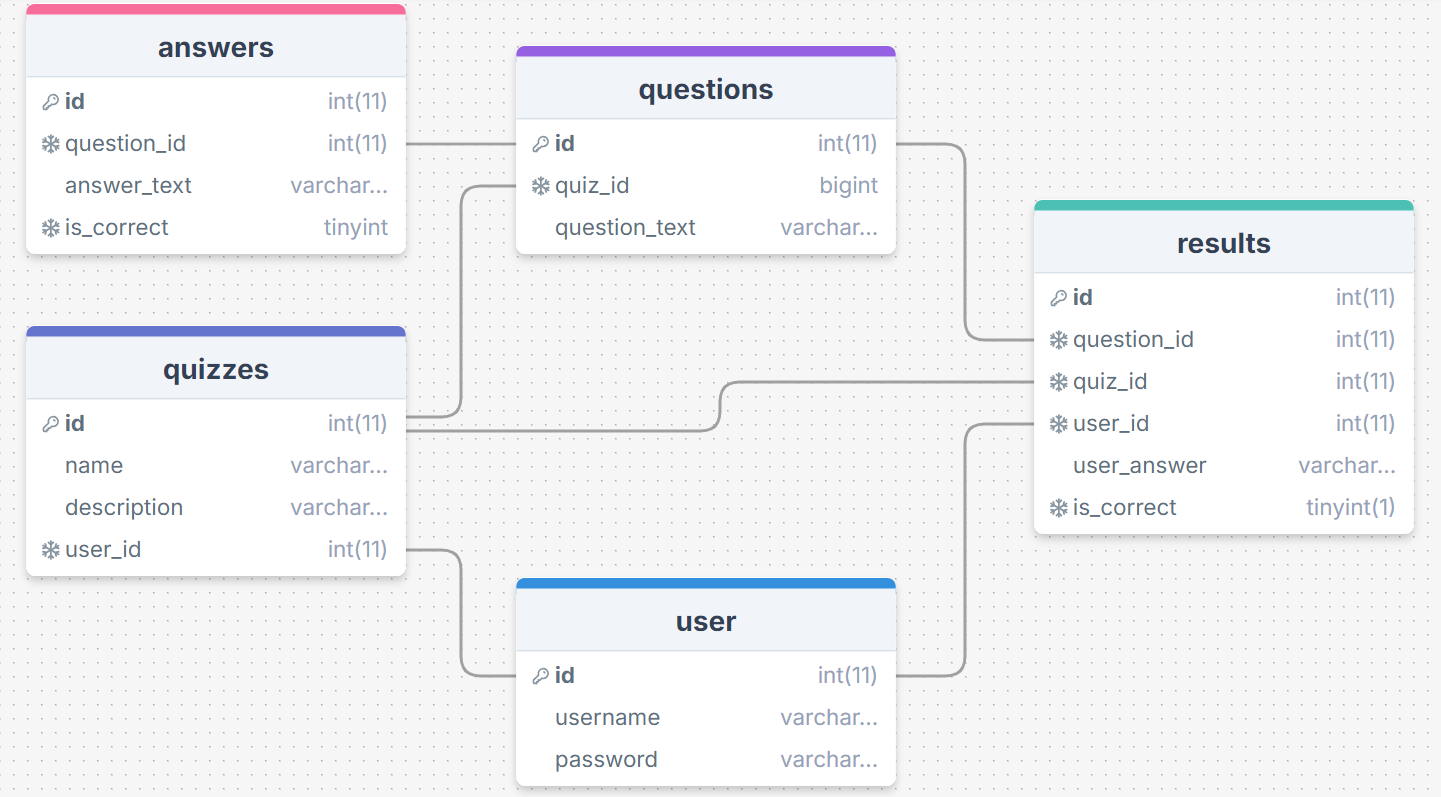
\includegraphics[width=0.8\textwidth]{img/db.png}}
		\caption{Схема базы данных}
		\label{db}
	\end{figure}

\newpage

\mysubsection{Определение обработчиков маршрутов}

В данной работе реализованы следующие обработчики маршрутов:
\begin{itemize}
    \item \lstinline|\user\:id| --- получение пользователя по id; 
    \item \lstinline|\login| --- проверка данных пользователя; 
    \item \lstinline|\addQuiz| --- добавление викторины; 
    \item \lstinline|\addQuestion\:quizId| --- добавление вопросов к викторине; 
    \item \lstinline|\getQuestionsByQuizId\:QuizId| --- получение вопрос по id викторины; 
    \item \lstinline|\deleteQuestion\:questionId| --- удаление вопроса по id; 
    \item \lstinline|\getAnswersByQuestionId\:questionId| --- поулчение ответов к вопросу по id вопроса; 
    \item \lstinline|\getQuizzesByUser\:userId| --- получение викторин созданных пользователем по id; 
    \item \lstinline|\deleteQuiz\:id| --- удаление викторины по id;
    \item \lstinline|\quizList| --- поулчение списка викторин;
    \item \lstinline|\getQuiz\:id| --- механизм прохождения викторины по id;
    \item \lstinline|\saveAnswer| --- сохранение ответа пользователя на вопрос;
    \item \lstinline|\deleteUserAnswers| --- удаление ответов пользователя на викторину;
    \item \lstinline|\results\:quizId| --- поулчение результатов прохождения викторины;
\end{itemize}


Обработчик маршрута для получения викторины по id представлен в листинге~\ref{listing1}.
\begin{lstlisting}[caption={Получение викторины по id}, label=listing1]
exports.getQuiz = async (req, res) => {
    try {
        const quizId = req.params.id;
        const quizz = await quiz.findByPk(quizId);
        const questions = await question.findAll({ where: { quiz_id: quizId } });
        const questionWithAnswers = await Promise.all(questions.map(async (question) => {
            const answers = await answer.findAll({ where: { question_id: question.id } });
            return {
                ...question.get(),
                answers
            };
        }));
        res.status(200).json({ quizz, questions: questionWithAnswers });
    } catch (error) {
        console.error(error);
        res.status(500).send({ message: "Ошибка при получении викторины." });
    }
};
\end{lstlisting} 


Обработчик маршрута для сохранения ответа пользователя~\ref{listing2}.
\begin{lstlisting}[caption={сохранение ответа пользователя}, label=listing2]
exports.saveAnswer = async (req, res) => {
    try {
        const user_id = req.userId;
        console.log(user_id);
      const {quiz_id, question_id, user_answer, is_correct } = req.body;
      console.log(req.body)        
      const newAnswer = await result.create({
        user_id,
        quiz_id,
        question_id,
        user_answer,
        is_correct
      });  
      return res.status(201).json({
        message: 'Ответ успешно сохранен!',
        answer: newAnswer
      });
    } catch (error) {
      console.error('Ошибка при сохранении ответа:', error);
      return res.status(500).json({ message: 'Ошибка сервера при сохранении ответа.' });
    }
  };
\end{lstlisting} 

Обработчик маршрута для получения вопросов викторины~\ref{listing3}.
\begin{lstlisting}[caption={сохранение ответа пользователя}, label=listing3]
exports.getQuestionsByQuizId = (req, res) => {
    const quizId = req.params.QuizId;
    console.log(req.params.QuizId)
    question.findAll({
        where: { quiz_id: quizId },
        include: [
            {
                model: answer,
                as: 'answers'
            }
        ]
    })
    .then(questions => {
        res.status(200).json(questions);
    })
    .catch(err => {
        globalFunctions.sendError(res, err);
    });
};
\end{lstlisting} 

В прил.~\ref{quizController.js} приведен код контроллера quizController.js.

В прил.~\ref{questionsController.js} приведен код для контроллера questionsController.js.

\mysubsection{Разработка компонентов}

При разработке приложения были созданы следующие компоненты:
\begin{itemize}
	\item AddQuestions.vue --- добавление вопросов к викторине; 
	\item AddQuiz.vue --- добавление викторины; 
	\item GoQuiz.vue --- прохождение викторины;
	\item MyQuiz.vue --- получение спсика викторин созданных пользователем;
	\item QuizList.vue --- получение списка викторин;
	\item QuizResult.vue --- получение результатов прохождения викторины;
	\item Login.vue --- получение логин страницы;
    \item Register.vue --- получение страницы регистраци.
\end{itemize}


\mysubsection{Реализованная функциональность}

Реализованная функциональность веб-приложения продемонстрирована далее в виде рисунков.

Осуществление авторизации происходит на странице, которая показана на рисунке~\ref{loginPage}.
\begin{figure}[!ht]
	\centering
	%Рамка только для изображений с белым фоном
	\fbox{
\includegraphics[width=1\textwidth]{img/login.png}}
	\caption{Страница авторизации}
	\label{loginPage}
\end{figure}

Просмотр списка викторин осуществляется на странице, которая показана на рисунке~\ref{quizList}.
\begin{figure}[!ht]
	\centering
	%Рамка только для изображений с белым фоном
	\fbox{
\includegraphics[width=1\textwidth]{img/quizList.png}}
	\caption{Список викторин}
	\label{quizList}
\end{figure}

Прохождение викторины реализовано на странице, которая показана на рисунке~\ref{quiz1} .
\begin{figure}[!ht]
	\centering
	%Рамка только для изображений с белым фоном
	\fbox{
\includegraphics[width=1\textwidth]{img/quiz1.png}}
	\caption{Прохождение викторины}
	\label{quiz1}
\end{figure}

Информация о правильных ответах выводится на странице, которая показана на рисунке~\ref{quiz2}.
\begin{figure}[!ht]
	\centering
	%Рамка только для изображений с белым фоном
	\fbox{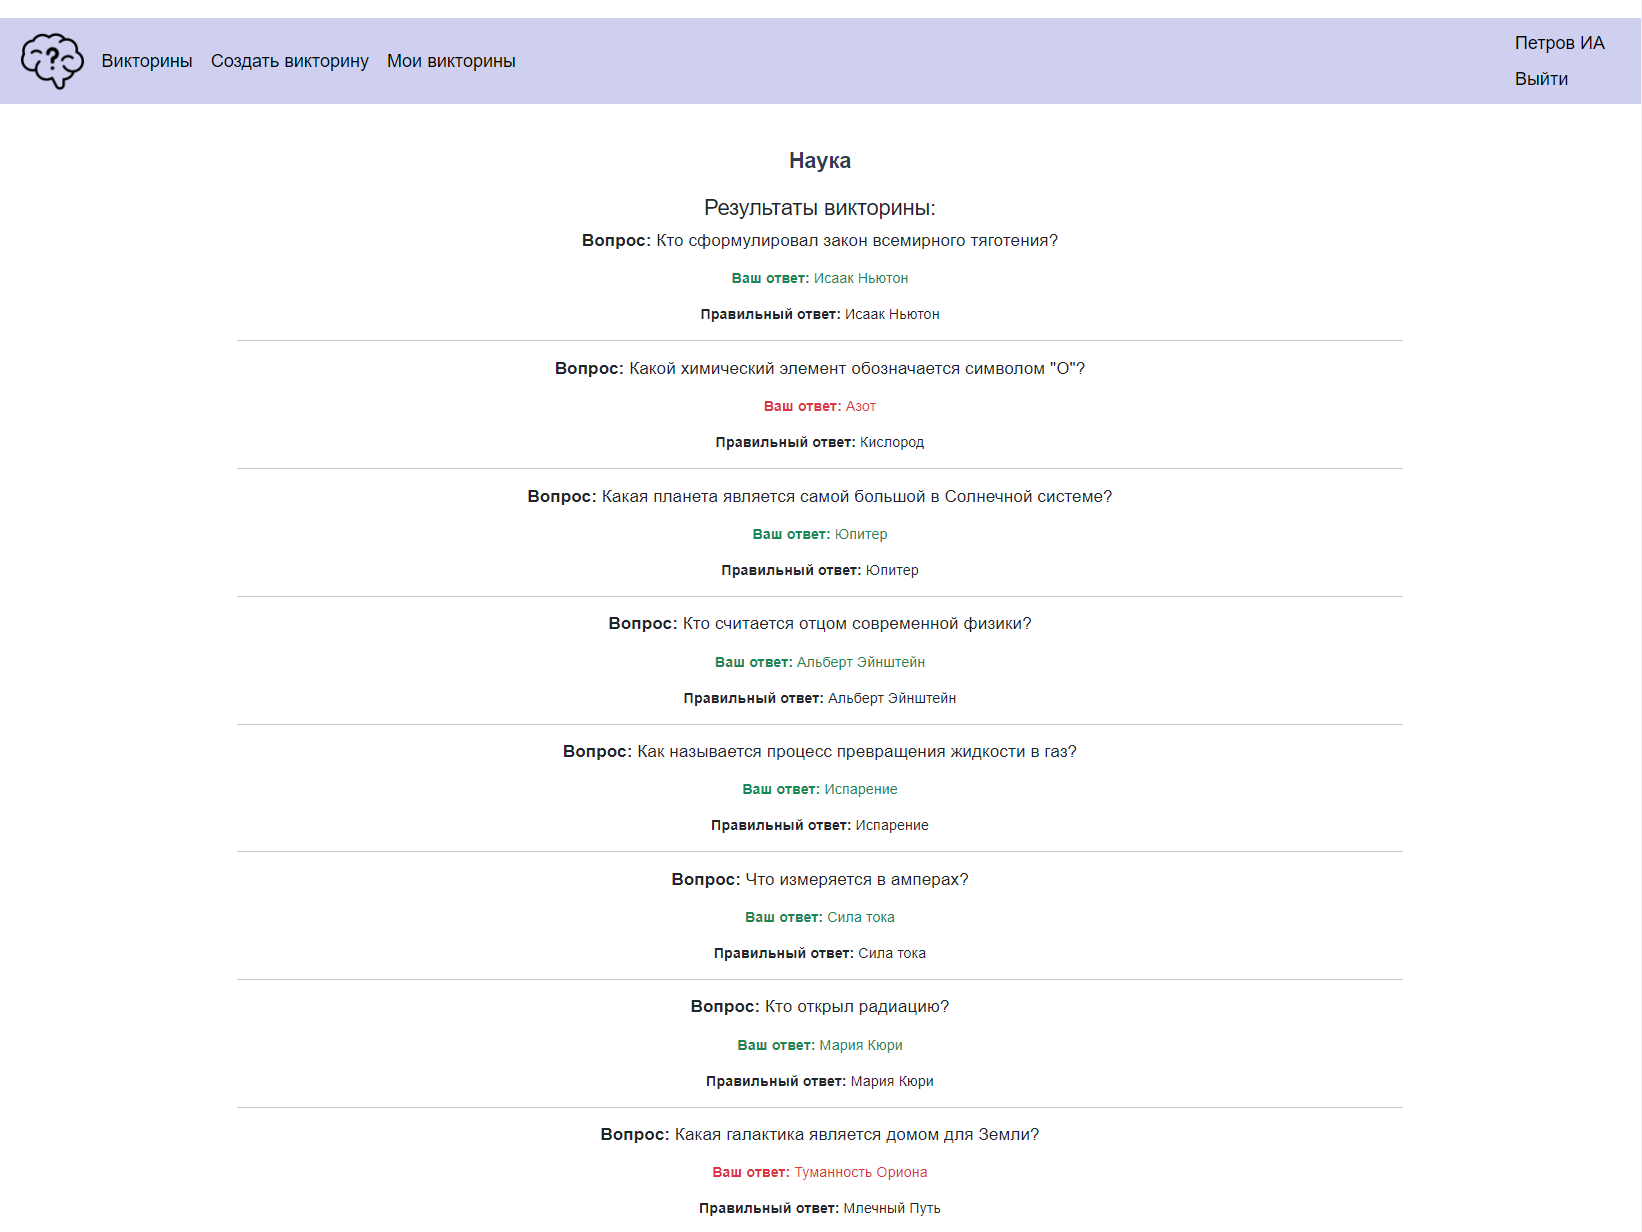
\includegraphics[width=0.9\textwidth]{img/quiz2.png}}
	\caption{Итоги викторины}
	\label{quiz2}
\end{figure}


\newpage
Ознакомиться с результатами прохождения викторины другими пользователями можно на странице, которая показана на рисунке~\ref{result}.
\begin{figure}[!ht]
	\centering
	%Рамка только для изображений с белым фоном
	\fbox{
\includegraphics[width=1\textwidth]{img/result.png}}
	\caption{Результаты викторины}
	\label{result}
\end{figure}

Добавление викторины реализовано на странице, которая показана на рисунке~\ref{newQuiz}.
\begin{figure}[!ht]
	\centering
	%Рамка только для изображений с белым фоном
	\fbox{
\includegraphics[width=1\textwidth]{img/newQuiz.png}}
	\caption{Создание викторины}
	\label{newQuiz}
\end{figure}

\newpage
Добавление вопросов в викторину реализовано на странице, которая показана на рисунке ~\ref{newQuest}.

\begin{figure}[!ht]
	\centering
	%Рамка только для изображений с белым фоном
	\fbox{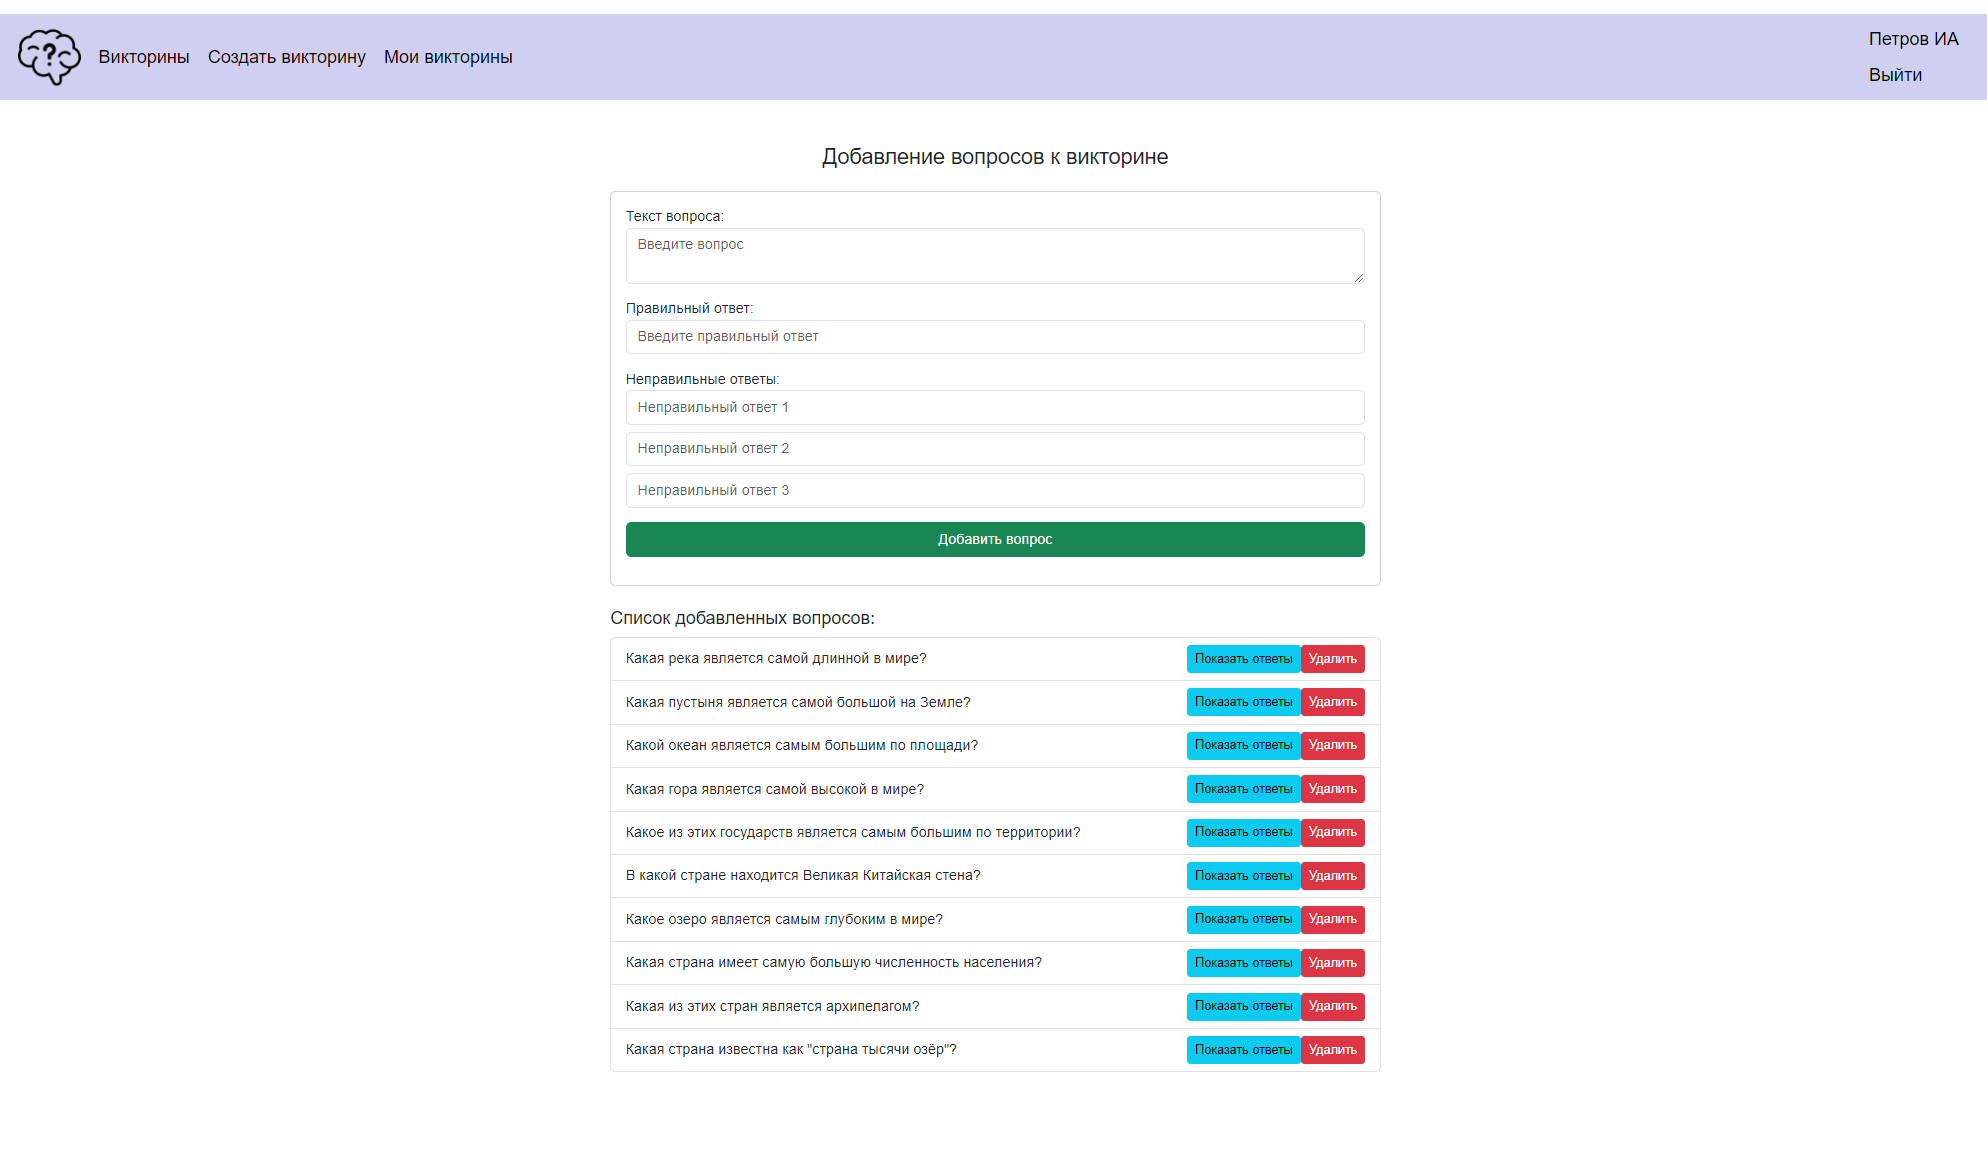
\includegraphics[width=1\textwidth]{img/newQuest.png}}
	\caption{Создание вопроса}
	\label{newQuest}
\end{figure}

Список викторин созданных пользователем показан на странице, которая показана на рисуке~\ref{MyQuiz}.

\begin{figure}[!ht]
	\centering
	%Рамка только для изображений с белым фоном
	\fbox{
\includegraphics[width=1\textwidth]{img/MyQuiz.png}}
	\caption{Ваши викторины}
	\label{MyQuiz}
\end{figure}

\mynonumbersection{ЗАКЛЮЧЕНИЕ}

В ходе выполнения курсовой работы было разработано веб-приложение для организации викторин.

Выполнены задачи:
\renewcommand{\labelenumii}{\alph{enumii})}
\begin{enumerate}[label={\arabic*)}]
	\item Разработана база данных;
	\item Созданы основные модули для перехода и просмотра объектов; 
    \item Разработано добавление и редактирование объектов;
	\item Разработано добавление викторин;
    \item Разработан просмотр пользователем всех доступных викторин и возможность пройти их.
    \item Разработан просматр результаты прохождения викторин.
\end{enumerate}

Выполнение перечисленных задач позволило достигнуть поставленную цель --- создать веб-приложение для организации викторин.

%-------------
%Список литературы
%-------------
\newpage
%Для включения в диплом списка литературы подключается файл lit.bib
%В нем приведены наиболее часто встречающиеся типы библиографических ссылок
\renewcommand{\refname}{СПИСОК ИСПОЛЬЗОВАННЫХ ИСТОЧНИКОВ}
\addcontentsline{toc}{section}{\refname}
\bibliography{lit}


\addappendix{Код контроллера quizController.js}
\label{quizController.js}
\begin{lstlisting}
var db = require('../config/db.config.js');
var globalFunctions = require('../config/global.functions.js');
var quiz = db.quiz1;
var question = db.question;
var answer = db.answer;
var result = db.result;
var user = db.user;
var result = db.result;
exports.create = (req, res) => {
    console.log(req.body);
    console.log(req.userId);
    quiz.create({
        id: req.body.id,
        name: req.body.name,
        description: req.body.description,
        user_id: req.userId,
    }).then(object => {
        globalFunctions.sendResult(res, object);
    }).catch(err => {
        globalFunctions.sendError(res, err);
    })
  };
  exports.findById = (req, res) => {
    quiz.findByPk(req.params.id)
        .then(object => {
            globalFunctions.sendResult(res, object);
        })
        .catch(err => {
            globalFunctions.sendError(res, err);
        })
  };  
exports.getQuizzesByUser = async (req, res) => {
    try {
        const userId = req.params.userId;
        if (!userId) {
            return res.status(400).json({ message: "User ID is required" });
        }

        const quizzes = await quiz.findAll({
            where: { user_id: req.userId } 
        });

        res.status(200).json(quizzes); 
    } catch (error) {
        console.error(error);
        res.status(500).json({ message: "Server error" });
    }
};
const deleteQuestion = async (questionId) => {
    return question.destroy({
        where: { id: questionId }
    });
};
const deleteResult = async (resultId) => {
    return result.destroy({
        where: {id: resultId }
    });
};
exports.deleteQuizWithQuestions = async (req, res) => {
    console.log(req.params);
    const quizId = req.params.id;
    try {
        const questions = await question.findAll({
            where: { quiz_id: quizId }
        });
        const results = await result.findAll({
            where: { quiz_id: quizId }
        });
        for (const question of questions) {
            await deleteQuestion(question.id);
        }
        for (const result of results) {
            await deleteResult(result.id);
        }
        await quiz.destroy({
            where: { id: quizId }
        });
        res.status(200).send({ message: "Викторина и все связанные с ней вопросы успешно удалены!" });
    } catch (err) {
        console.error(err);
        res.status(500).send({ message: "Произошла ошибка при удалении викторины и вопросов." });
    }
};
exports.getAllQuizzes = async (req, res) => {
    try {
        const quizzes = await quiz.findAll();
        res.status(200).json(quizzes);
    } catch (error) {
        console.error(error);
        res.status(500).send({ message: "Ошибка при получении викторин." });
    }
};
exports.getQuiz = async (req, res) => {
    try {
        const quizId = req.params.id;
        const quizz = await quiz.findByPk(quizId);
        const questions = await question.findAll({ where: { quiz_id: quizId } });
        const questionWithAnswers = await Promise.all(questions.map(async (question) => {
            const answers = await answer.findAll({ where: { question_id: question.id } });
            return {
                ...question.get(),
                answers
            };
        }));
        res.status(200).json({ quizz, questions: questionWithAnswers });
    } catch (error) {
        console.error(error);
        res.status(500).send({ message: "Ошибка при получении викторины." });
    }
};
exports.submitResults = async (req, res) => {
    console.log(req.body);
    const { userId, quizId, results } = req.body;
    try { 
        const quizz = await quiz.findByPk(quizId);
        if (!quizz) {
            return res.status(404).json({ message: 'Викторина не найдена' });
        }   
        const saveResultsPromises = results.map(result => {
            return Result.create({
                user_id: userId,
                quiz_id: quizId,
                question_id: result.questionId,
                user_answer: result.userAnswer,
                is_correct: result.isCorrect
            });
        });
        await Promise.all(saveResultsPromises);
        res.status(200).json({ message: 'Результаты успешно сохранены' });
    } catch (error) {
        console.error('Ошибка при сохранении результатов:', error);
        res.status(500).json({ message: 'Ошибка сервера' });
    }
};
exports.saveAnswer = async (req, res) => {
    try {
        const user_id = req.userId;
        console.log(user_id);
      const {quiz_id, question_id, user_answer, is_correct } = req.body;
      console.log(req.body)        
      const newAnswer = await result.create({
        user_id,
        quiz_id,
        question_id,
        user_answer,
        is_correct
      });
      return res.status(201).json({
        message: 'Ответ успешно сохранен!',
        answer: newAnswer
      });
    } catch (error) {
      console.error('Ошибка при сохранении ответа:', error);
      return res.status(500).json({ message: 'Ошибка сервера при сохранении ответа.' });
    }
  };
exports.deleteUserAnswers = async (req, res) => {
    console.log("gggg");
    const userId = req.userId;
    const quizId = req.body.quizId;
    console.log(userId);
    console.log(quizId);
    try {   
      await result.destroy({
        where: {
          user_id: userId,
          quiz_id: quizId
        }
      });
      res.status(200).json({ message: 'Ответы успешно удалены.' });
    } catch (error) {
      console.error('Ошибка при удалении ответов:', error);
      res.status(500).json({ error: 'Ошибка при удалении ответов.' });
    }
};
exports.getResults = async (req, res) => {
    const quizId = req.params.quizId;
    const currentUserId = req.userId;
    try { 
        const results = await result.findAll({
            where: { quiz_id: quizId },
            attributes: ['user_id', 'is_correct'],
        });
        const userIds = [...new Set(results.map(result => result.user_id))];
        const users = await user.findAll({
            where: {
                id: userIds
            },
            attributes: ['id', 'username']
        });
        const userMap = {};
        users.forEach(user => {
            userMap[user.id] = user.username;
        }); 
        const userResults = {};
        results.forEach(answer => {
            const userId = answer.user_id;
            const userName = userMap[userId];   
            if (!userResults[userId]) {
                userResults[userId] = {
                    userId: userId,
                    userName: userName,
                    correctAnswers: 0,
                    totalAnswers: 0
                };
            }   
            userResults[userId].totalAnswers += 1;
            if (answer.is_correct) {
                userResults[userId].correctAnswers += 1;
            }
        }); 
        const responseResults = Object.values(userResults);
        responseResults.sort((a, b) => b.correctAnswers - a.correctAnswers);
        return res.status(200).json({ results: responseResults, currentUserId });
    } catch (error) {
        console.error('Ошибка при получении результатов:', error);
        res.status(500).json({ error: 'Ошибка при получении результатов.' });
    }
};
\end{lstlisting}



\addappendix{Код контроллера questionsController.js}
\label{questionsController.js}
\begin{lstlisting}
var db = require('../config/db.config.js');
var globalFunctions = require('../config/global.functions.js');
var question = db.question;
var answer = db.answer;
var quiz = db.quiz1;
exports.create = async (req, res) => {
    try {
        console.log(req.body);
        const createdQuestion = await question.create({
            quiz_id: req.body.quiz_id,
            question_text: req.body.question_text
        });
        const questionId = createdQuestion.id;
        await answer.create({
            question_id: questionId,
            answer_text: req.body.correctAnswer,
            is_correct: true
        });
        await answer.bulkCreate([
            {
                question_id: questionId,
                answer_text: req.body.wrongAnswer1,
                is_correct: false
            },
            {
                question_id: questionId,
                answer_text: req.body.wrongAnswer2,
                is_correct: false
            },
            {
                question_id: questionId,
                answer_text: req.body.wrongAnswer3,
                is_correct: false
            }
        ]);

        globalFunctions.sendResult(res, {
            message: "Вопрос и ответы успешно добавлены!"
        });
    } catch (err) {
        console.error("Ошибка при добавлении вопроса и ответов:", err);

        globalFunctions.sendError(res, err);
    }
};
exports.getQuestionsByQuizId = (req, res) => {
    const quizId = req.params.QuizId;
    console.log(req.params.QuizId)
    question.findAll({
        where: { quiz_id: quizId },
        include: [
            {
                model: answer,
                as: 'answers'
            }
        ]
    })
    .then(questions => {
        res.status(200).json(questions);
    })
    .catch(err => {
        globalFunctions.sendError(res, err);
    });
};
exports.deleteQuestion = (req, res) => {
    console.log(req.params);
    const questionId = req.params.questionId;
    console.log(req.params.questionId)
    question.destroy({
        where: { id: questionId }
    })
    .then(() => {
        res.status(200).send({ message: "Вопрос успешно удалён!" });
    })
    .catch(err => {
        globalFunctions.sendError(res, err);
    });
};
exports.getAnswersByQuestionId = (req, res) => {
    const questionId = req.params.questionId;
    console.log(req.params.questionId)
    answer.findAll({
        where: { question_id: questionId }
    })
    .then(answers => {
        res.json(answers);
    })
    .catch(err => {
        console.error(err);
        res.status(500).json({ error: 'Ошибка при получении ответов.' });
    });
};
exports.findAll = (req, res) => {
    question.findAll()
    .then(objects => {
     globalFunctions.sendResult(res, objects);
     })
     .catch(err => {
         globalFunctions.sendError(res, err);
     })
 };
\end{lstlisting}

\end{document}

